\documentclass{article}
\usepackage[utf8]{inputenc}
\usepackage[spanish]{babel}
\usepackage{pdfpages}
\usepackage{listings}
\usepackage{graphicx}
\usepackage{float}

%\usepackage{mips}

\setlength{\parskip}{1ex plus 0.5ex minus 0.2ex}
\title{Trabajo Práctico 1} 
\author{
  Agustin Alejandro Linari, \textit{Padrón Nro. 81.783}\\
  \textit{agustinlinari@gmail.com}\\
  \and
  Juan Ignacio López Pecora, \textit{Padrón Nro. 84.700}\\
  \textit{jlopezpecora@gmail.com}\\
  \and
  Pablo Daniel Sívori, \textit{Padrón: 84.026}\\
  \textit{sivoridaniel@gmail.com}\\
  \\
  \normalsize{2$^{\circ}$ Cuatrimestre de 2016}                           \\
  \normalsize{66.20 Organizacion de Computadoras}                  \\
  \normalsize{Facultad de Ingenieria, Universidad de Buenos Aires} \\
}

%\newcommand{\ip}[2]{(#1, #2)}
                             % Defines \ip{arg1}{arg2} to mean
                             % (arg1, arg2).

%\newcommand{\ip}[2]{\langle #1 | #2\rangle}
                             % This is an alternative definition of
                             % \ip that is commented out.

\begin{document}             % End of preamble and beginning of text.

%\maketitle                   % Produces the title.
\maketitle


\begin{abstract}
En el presente trabajo utilizamos el conjunto de instrucciones MIPS y el concepto de ABI para resolver parte de la lógica del programa realizado en el trabajo práctico 0. 
\end{abstract}

\clearpage

\tableofcontents
\clearpage

\part{Desarrollo}

\section{Introduccion}

El objetivo del presente trabajo práctico es familiarizarse con el código de instrucciones MIPS 32. Para ello implementaremos la lógica de cómputo del fractal con dicho código de instrucciones. 
Finalmente compilaremos el programa en el emulador GXemul para poder obtener el código de instrucciones Mips32.

\section{Build}
El correspondiente informe se puede construir utilizando el make con la etiqueta doc la cual borra y genera el informe en formato pdf.

\section{Diseño e Implementación del Programa}

El código fuente del programa se puede encontrar en el anexo \ref{sec:source}.

\subsection{Stack Frame}
A continuación mostramos los diagrama de stack frame de las funciones implementadas en MIPS32.

\begin{figure}[H]
	\centering
		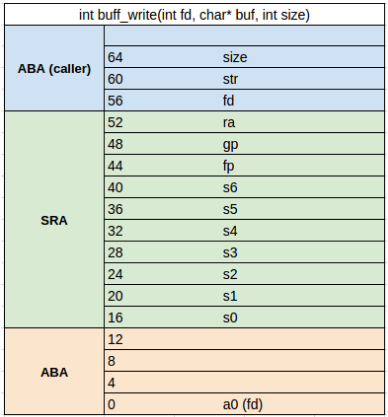
\includegraphics[scale=0.4]{stack1.png}
	\caption{Stack1}
	\label{fig:stack1}
\end{figure}

\begin{figure}[H]
	\centering
		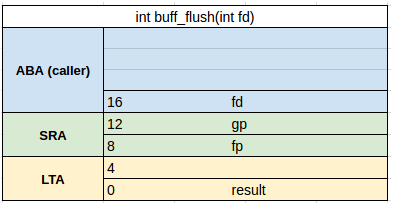
\includegraphics[scale=0.4]{stack2.png}
	\caption{Stack2}
	\label{fig:stack2}
\end{figure}

\begin{figure}[H]
	\centering
		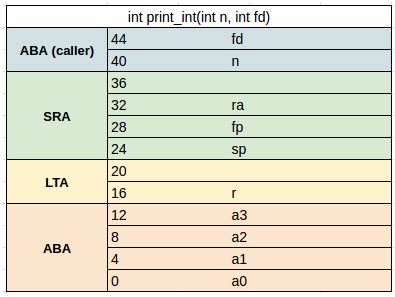
\includegraphics[scale=0.4]{stack3.png}
	\caption{Stack3}
	\label{fig:stack3}
\end{figure}

\begin{figure}[H]
	\centering
		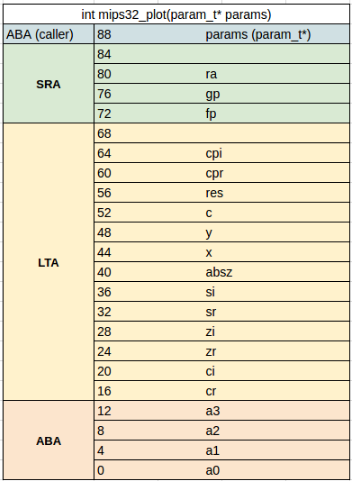
\includegraphics[scale=0.4]{stack4.png}
	\caption{Stack4}
	\label{fig:stack4}
\end{figure}


\section{Corridas de Programa}

\subsection{Ejemplos}

\subsection{Pruebas}

\clearpage

\section{Análisis}

\textbf{\textit{Mediciones}}

\begin{itemize}
\item[•] Todos los programas fueron compilados con el parámetro -O0 (sin optimizaciones).\\
\item[•] Todas las mediciones corresponden a la ejecución de los programas utilizando el comando time.\\
\end{itemize}


\begin{table}[htbp]
\begin{center}
\begin{tabular}{|l|l|l|l|}
\hline
Código C & real & usr & sys \\
\hline \hline
1 & 1m19.363s & 1m19.143s & 0m0.141s \\ \hline
2 & 1m23.195s & 1m23.014s & 0m0.129s \\ \hline
3 & 1m21.480s & 1m19.335s & 0m0.133s \\ \hline
promedio & 1m 21.346s & 1m 20.497s & 0.134s
\end{tabular}
\caption{Tiempos promedios de ejecución en código C.}
\end{center}
\end{table}

\begin{table}[htbp]
\begin{center}
\begin{tabular}{|l|l|l|l|}
\hline
Código C & real & usr & sys \\
\hline \hline
1 & 1m0.449s & 0m52.722s & 0m7.680s \\ \hline
2 & 1m0.879s & 0m53.042s & 0m7.808s \\ \hline
3 & 1m1.246s & 0m53.261s & 0m7.937s \\ \hline
promedio & 1m0.858s & 53.008s & 7.808s
\end{tabular}
\caption{Tiempos promedios de ejecución en código Mips buffer size 64 bytes.}
\end{center}
\end{table}

\begin{table}[htbp]
\begin{center}
\begin{tabular}{|l|l|l|l|}
\hline
Código C & real & usr & sys \\
\hline \hline
1 & 1m4.262s & 1m3.237s & 0m0.984s \\ \hline
2 & 1m1.246s & 1m0.319s & 0m0.883s \\ \hline
3 & 0m58.547s & 0m57.573s & 0m0.937s \\ \hline
promedio & 1m1.352s & 1m0.376s & 0.935s
\end{tabular}
\caption{Tiempos promedios de ejecución en código Mips buffer size 1 KB.}
\end{center}
\end{table}

\begin{table}[htbp]
\begin{center}
\begin{tabular}{|l|l|l|l|}
\hline
Código C & real & usr & sys \\
\hline \hline
1 & 1m3.797s & 1m3.589s & 0m0.156s \\ \hline
2 & 1m0.617s & 1m0.480s & 0m0.133s \\ \hline
3 & 1m4.500s & 1m4.249s & 0m0.215s \\ \hline
promedio & 1m2.971s & 1m2.772s & 0.168s
\end{tabular}
\caption{Tiempos promedios de ejecución en código Mips buffer size 16 KB.}
\end{center}
\end{table}

\clearpage

\begin{center}
\textit{\textbf{Representamos gráficamente los valores obtenidos en los cuadros anteriores, y hacemos una comparación entre los tiempos promedios de ejecución obtenidos en cada código}}
\end{center}

\begin{figure}[H]
	\centering
		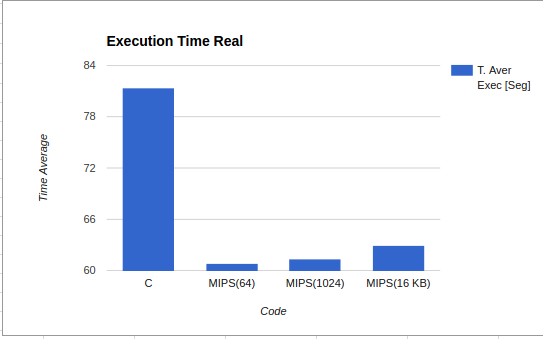
\includegraphics[scale=0.6]{TPromExecReal.png}
\end{figure}
\begin{figure}[H]
	\centering
	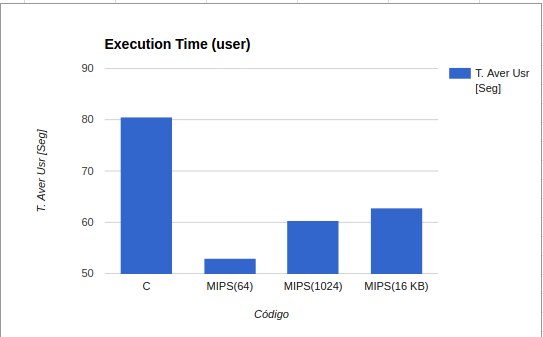
\includegraphics[scale=0.6]{TPromExecUsr.png}
\end{figure}
\begin{figure}[H]
	\centering
		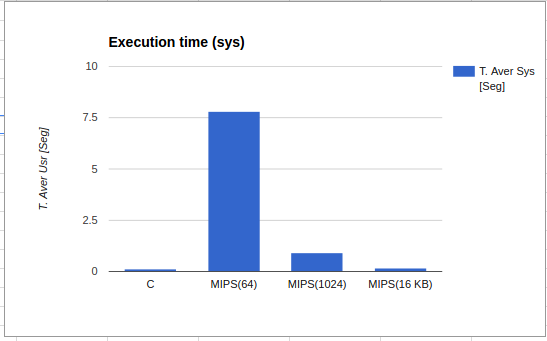
\includegraphics[scale=0.6]{TPromExecSys.png}
\end{figure}


\clearpage


\begin{table}[htbp]
\begin{center}
\begin{tabular}{|l|l|}
\hline
Speed Up & Value \\
\hline \hline
tc / tmips 64B & 1.34 \\ \hline
tc / tmips 1KB & 1.33 \\ \hline
tc / tmips 16KB & 1.29 \\ \hline

\end{tabular}
\caption{Speed UP}
\end{center}
\end{table}

\textbf{\textit{Observaciones}}

\begin{itemize}
\item[•] La implementación de mips en cualquiera de sus variantes se ejecuta en menos tiempo que la implementación C pura, con un speed up aproximado de 1/3.\\
\item[•] A medida que el buffer se agranda, el tiempo de sistema se reduce. Esto se debe a que se producen menos syscalls a write.\\
\item[•] Podemos plantear la hipótesis razonable de que printf está implementada con un buffer (debido al bajo sys time). Para nuestra implementación MIPS, el tamaño del buffer que obtuvo un tiempo sys del mismo orden que la implementación C fue de 16 KB.\\
\item[•] Contrario a lo que nuestra intuición indicaba, aumentar el buffer para valores mayores a 64 bytes no necesariamente significó (en promedio) en un aumento de performance. Esto puede estar relacionado con la arquitectura del cache emulado, el tamaño de bloque  y su política de reemplazo.\\
\end{itemize}

\clearpage

\section{Conclusiones}

Con la realización de este trabajo hemos podido apreciar la diferencia de performance entre dos implementaciones de distinta naturaleza de un mismo algoritmo, implementado en C y en assembly MIPS32.\\
\\
A la hora de programar, es común que se codifique utilizando lenguajes de alto nivel. El lenguaje de programación C es un lenguaje de propósito general clásico cuyo diseño provee construcciones que mapean de manera eficiente instrucciones de máquina típicas. Las ventajas de utilizar un lenguaje de alto nivel como C son portabilidad (a nivel código fuente) entre diferentes arquitecturas donde se haya implementado el compilador, aumento de productividad - dado que se abstrae de cuestiones de bajo nivel íntimamente ligadas con la arquitectura de la máquina - y reducción en el costo de mantenimiento. Sin embargo, estas ventajas traen aparejado un costo en la performance del programa.\\
\\
En algunos casos, los requerimientos funcionales de un programa requieren de una performance que puede ser difícil de alcanzar para una implementación en un lenguaje de alto nivel. Mediante un análisis cuantitativo, se determina qué segmentos de código consumen la mayor cantidad de recursos de una computadora -ciclos de CPU, memoria, etc-. Para el caso particular de este trabajo, la función de cómputo del fractal es central en el desempeño de la aplicación.\\
\\
Aprovechando la posibilidad que brinda el lenguaje C de poder linkear con código assembly, pudimos implementar las funciones clave a medida de la computadora, esto es, codificar utilizando el conjunto de instrucciones de la arquitectura MIPS32, dando como resultado un desempeño superior reflejado en el cálculo del Speed Up.\\
\\
Podemos concluir que ante requerimientos que condicionen el uso de recursos de una computadora, o la necesidad de proveer una aplicación donde la velocidad de ejecución sea un requerimiento clave, podemos obtener lo mejor de dos mundos, implementando la aplicación en un lenguaje de alto nivel y optimizando los segmentos de código clave implementando en assembly para la arquitectura sobre la cual se ejecutará la aplicación.\\
\\
Finalmente, vale la pena observar que en un contexto diferente, si dejamos de forzar al compilador C (GCC) a no optimizar el código, se puede dar el caso que el código C compilado, libre de restricciones de optimización, pueda superar el rendimiento de una implementación MIPS hecha por nosotros, debido a la madurez alcanzada de los compiladores modernos y nuestra inexperiencia en la implementación de código assembler.

\clearpage

\part{Apendice}
\appendix


\section{Codigo fuente}\label{sec:source}
\definecolor{gray}{rgb}{0.5,0.5,0.5}
\lstset{%
  title=\lstname,
  language=C,
  basicstyle=\footnotesize,
  showspaces=false,
  showstringspaces=false,
  breaklines=true,
  commentstyle=\color{gray},
  numbers=left,
  numberstyle=\tiny\color{gray},
  numbersep=5pt,
  frame=single
}

%\lstinputlisting{../src/complex.h}
%\lstinputlisting{../src/complex.c}
%\lstinputlisting{../src/app.c}

\clearpage

%\lstinputlisting{../MIPS32/complex.s}
%\lstinputlisting{../MIPS32/app.s}

\clearpage

\section{Enunciado original}\label{sec:enunciado}
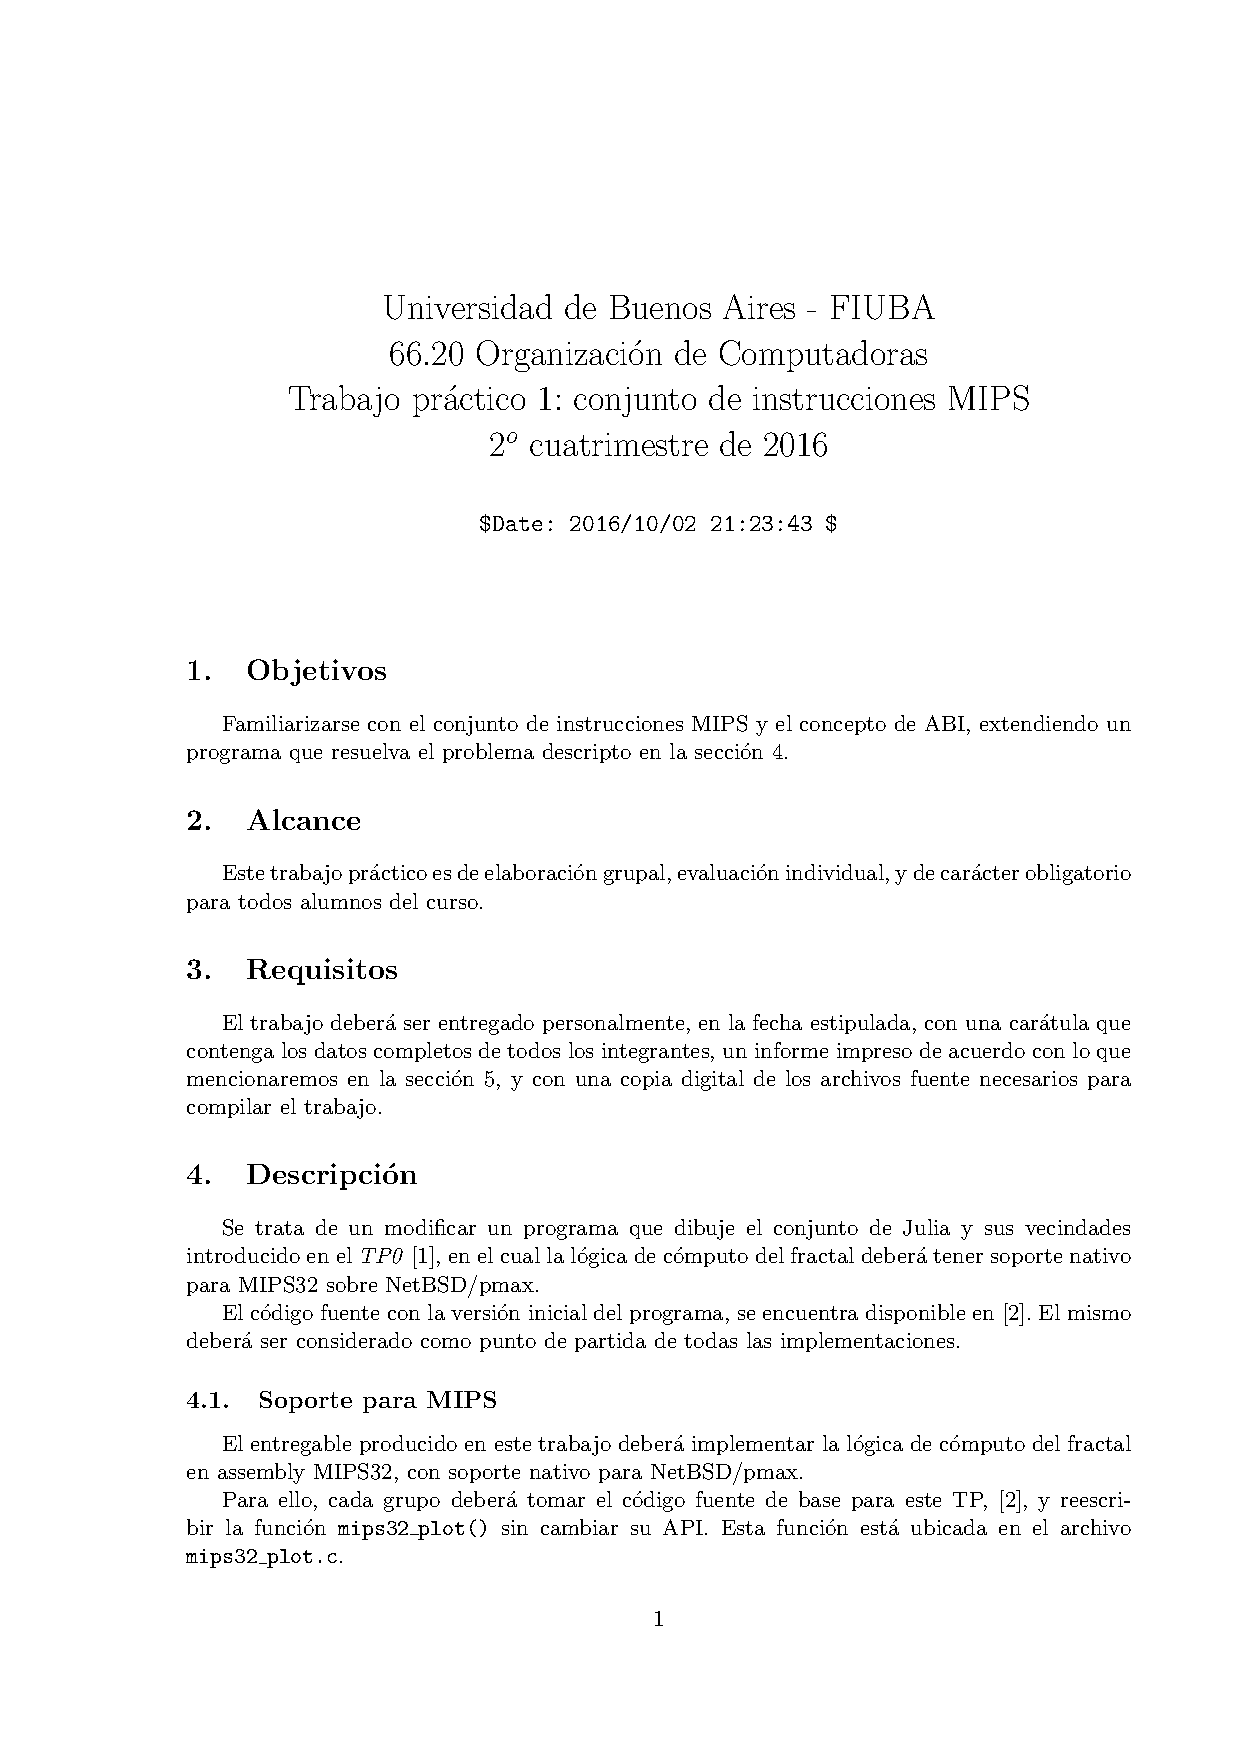
\includepdf[pages={-}]{tp1-2016-2q.pdf}

\end{document}               % End of document.
